
\documentclass[a4paper,11pt]{article}
\usepackage[a4paper, margin=8em]{geometry}

% usa i pacchetti per la scrittura in italiano
\usepackage[french,italian]{babel}
\usepackage[T1]{fontenc}
\usepackage[utf8]{inputenc}
\frenchspacing 

% usa i pacchetti per la formattazione matematica
\usepackage{amsmath, amssymb, amsthm, amsfonts}

% usa altri pacchetti
\usepackage{gensymb}
\usepackage{hyperref}
\usepackage{standalone}

% imposta il titolo
\title{Appunti Fondamenti di Automatica}
\author{Luca Seggiani}
\date{2025}

% disegni
\usepackage{pgfplots}
\pgfplotsset{width=10cm,compat=1.9}

% imposta lo stile
% usa helvetica
\usepackage[scaled]{helvet}
% usa palatino
\usepackage{palatino}
% usa un font monospazio guardabile
\usepackage{lmodern}

% tikz in sans
\tikzset{every picture/.style={/utils/exec={\sffamily}}}

\renewcommand{\rmdefault}{ppl}
\renewcommand{\sfdefault}{phv}
\renewcommand{\ttdefault}{lmtt}

% circuiti
\usepackage{circuitikz}
\usetikzlibrary{babel}

% disponi il titolo
\makeatletter
\renewcommand{\maketitle} {
	\begin{center} 
		\begin{minipage}[t]{.8\textwidth}
			\textsf{\huge\bfseries \@title} 
		\end{minipage}%
		\begin{minipage}[t]{.2\textwidth}
			\raggedleft \vspace{-1.65em}
			\textsf{\small \@author} \vfill
			\textsf{\small \@date}
		\end{minipage}
		\par
	\end{center}

	\thispagestyle{empty}
	\pagestyle{fancy}
}
\makeatother

% disponi teoremi
\usepackage{tcolorbox}
\newtcolorbox[auto counter, number within=section]{theorem}[2][]{%
	colback=blue!10, 
	colframe=blue!40!black, 
	sharp corners=northwest,
	fonttitle=\sffamily\bfseries, 
	title=Teorema~\thetcbcounter: #2, 
	#1
}

% disponi definizioni
\newtcolorbox[auto counter, number within=section]{definition}[2][]{%
	colback=red!10,
	colframe=red!40!black,
	sharp corners=northwest,
	fonttitle=\sffamily\bfseries,
	title=Definizione~\thetcbcounter: #2,
	#1
}

% disponi problemi
\newtcolorbox[auto counter, number within=section]{problem}[2][]{%
	colback=green!10,
	colframe=green!40!black,
	sharp corners=northwest,
	fonttitle=\sffamily\bfseries,
	title=Problema~\thetcbcounter: #2,
	#1
}

% disponi codice
\usepackage{listings}
\usepackage[table]{xcolor}

\lstdefinestyle{codestyle}{
		backgroundcolor=\color{black!5}, 
		commentstyle=\color{codegreen},
		keywordstyle=\bfseries\color{magenta},
		numberstyle=\sffamily\tiny\color{black!60},
		stringstyle=\color{green!50!black},
		basicstyle=\ttfamily\footnotesize,
		breakatwhitespace=false,         
		breaklines=true,                 
		captionpos=b,                    
		keepspaces=true,                 
		numbers=left,                    
		numbersep=5pt,                  
		showspaces=false,                
		showstringspaces=false,
		showtabs=false,                  
		tabsize=2
}

\lstdefinestyle{shellstyle}{
		backgroundcolor=\color{black!5}, 
		basicstyle=\ttfamily\footnotesize\color{black}, 
		commentstyle=\color{black}, 
		keywordstyle=\color{black},
		numberstyle=\color{black!5},
		stringstyle=\color{black}, 
		showspaces=false,
		showstringspaces=false, 
		showtabs=false, 
		tabsize=2, 
		numbers=none, 
		breaklines=true
}

\lstdefinelanguage{javascript}{
	keywords={typeof, new, true, false, catch, function, return, null, catch, switch, var, if, in, while, do, else, case, break},
	keywordstyle=\color{blue}\bfseries,
	ndkeywords={class, export, boolean, throw, implements, import, this},
	ndkeywordstyle=\color{darkgray}\bfseries,
	identifierstyle=\color{black},
	sensitive=false,
	comment=[l]{//},
	morecomment=[s]{/*}{*/},
	commentstyle=\color{purple}\ttfamily,
	stringstyle=\color{red}\ttfamily,
	morestring=[b]',
	morestring=[b]"
}

% disponi sezioni
\usepackage{titlesec}

\titleformat{\section}
	{\sffamily\Large\bfseries} 
	{\thesection}{1em}{} 
\titleformat{\subsection}
	{\sffamily\large\bfseries}   
	{\thesubsection}{1em}{} 
\titleformat{\subsubsection}
	{\sffamily\normalsize\bfseries} 
	{\thesubsubsection}{1em}{}

% disponi alberi
\usepackage{forest}

\forestset{
	rectstyle/.style={
		for tree={rectangle,draw,font=\large\sffamily}
	},
	roundstyle/.style={
		for tree={circle,draw,font=\large}
	}
}

% disponi algoritmi
\usepackage{algorithm}
\usepackage{algorithmic}
\makeatletter
\renewcommand{\ALG@name}{Algoritmo}
\makeatother

% disponi numeri di pagina
\usepackage{fancyhdr}
\fancyhf{} 
\fancyfoot[L]{\sffamily{\thepage}}

\makeatletter
\fancyhead[L]{\raisebox{1ex}[0pt][0pt]{\sffamily{\@title \ \@date}}} 
\fancyhead[R]{\raisebox{1ex}[0pt][0pt]{\sffamily{\@author}}}
\makeatother

\begin{document}

% sezione (data)
\section{Lezione del 05-03-25}

% stili pagina
\thispagestyle{empty}
\pagestyle{fancy}

% testo
Avevamo visto la forma standard per sistemi lineari:
\[
	\begin{cases}
		x' = Ax + Bx \\
		y = Cx + Du \\
		x(0) = x_0
	\end{cases}
\]
(con $D$ solitamente nulla), e la soluzione data da:
\[
	\begin{cases}
		x(t) = e^{At} x_0 + \int_0^t e^{A(t - \tau)} Bu(\tau) d\tau \\
		y(t) = Ce^{At} x_0 + C\int_0^t e^{A(t - \tau)} Bu(\tau) d\tau + Du \\
	\end{cases}
\]

per il calcolo di tale soluzione sfruttavamo l'\textit{esponenziale di matrice:}
$$
e^{At} = I + At + \frac{1}{2}A^2t^2+ ... + \frac{(At)^n}{n!} = \sum_{k = 0}^{+\infty} \frac{(At)^k}{k!} 
$$

Abbiamo visto che se la matrice $A$ ha autovalori distinti, allora è diagonalizzabile:
$$
A = T^{-1} A_D T, \quad A_D = \begin{pmatrix}
	\lambda_1 & 0 & 0 \\
	0 & ... & 0 \\
	0 & 0 & \lambda_n \\
\end{pmatrix}
$$
e l'esponenziale di matrice è semplice:
$$
e^{At} = T^{-1} e^{A_D t} T = T^{-1} \begin{pmatrix}
	e^{\lambda_1 t} & 0 & 0 \\
	0 & ... & 0 \\
	0 & 0 & e^{\lambda_n t} \\
\end{pmatrix} T
$$

In particolare, se gli autovalori sono complessi e coniugati, si avrà:
$$
\lambda_i = \sigma_i + j \omega_i, \quad \overline{\lambda_i} = \sigma_i - j \omega_i 
$$
da cui:
$$
e^{\lambda_i t} = e^{\sigma_i t} e^{j\omega_i t}, \quad e^{\overline{\lambda_i} t} = e^{\sigma_i t} e^{-j\omega_i t}
$$
e si avranno quindi modi oscillatori ed esponenziali.

Avevamo inoltre definito come \textbf{modi propri} associati i:
$$
C(t) e^{\lambda t} = C(t) = \alpha_0 + \alpha_1 + \alpha_2 t^2 + ... + \alpha_{k - 1} t^{k -1}
$$

\subsubsection{Matrice reale, autovalori complessi}
Se $A$ è reale ma i suoi autovalori sono complessi, si avra una forma del tipo:
$$
A_D = \begin{pmatrix}
	\sigma + j\omega & 0 \\
	0 & \sigma - j\omega
\end{pmatrix}
$$

Questa forma è \textit{simile} alla matrice reale $S$:
$$
S = \begin{pmatrix}
	\sigma & \omega \\
	-\omega & \sigma
\end{pmatrix}
$$

\subsubsection{Calcolo degli autovalori}
Ripassiamo brevemente come calcolare gli autovalori.
Se $V$ è autovettore e $\lambda$ l'autovalore associato, allora vale:
$$
Av = \lambda v \implies (A - \lambda I)v = 0 \implies \mathrm{det} (A - \lambda I) = 0
$$
detta \textbf{equazione caratteristica} $p(\lambda)$: 
$$
p(\lambda) = \mathrm{det} (A - \lambda I) = \lambda^n + \alpha_1 \lambda^{n - 1} + \alpha_2 \lambda^{n - 2} + ... + \alpha_{n - 1} \lambda + \alpha_n
$$

Avremo quindi che le soluzioni di $\lambda^*$ di $p(\lambda) = 0$ rappresentano gli autovalori di $A$.

\subsubsection{Esempio: soluzione di differenziale con derivata prima dell'ingresso}
Avevamo visto l'equazione differenziale (esempio 4.2.2):
$$
y'' + y = 2u + u'
$$
da cui avevamo ricavato il sistema:
\[
	\begin{cases}
		\begin{pmatrix}
			x_1' \\ x_2'
		\end{pmatrix}
		=
		\begin{pmatrix}
			0 & 1 \\ 
			-1 & 0
		\end{pmatrix}
		\begin{pmatrix}
			x_1 \\ x_2
		\end{pmatrix}
		+
		\begin{pmatrix}
		0 \\ 1
		\end{pmatrix}
		u \\ 

		y = 
		\begin{pmatrix}
			2 & 1
		\end{pmatrix}
		\begin{pmatrix}
			x_1 \\ x_2
		\end{pmatrix}
		+
		\begin{pmatrix}
			0
		\end{pmatrix}
		u
	\end{cases}
\]
Abbiamo quindi le matrici:
$$
	A = \begin{pmatrix}
			0 & 1 \\ 
			-1 & 0
		\end{pmatrix}, \quad 
	B = \begin{pmatrix}
		0 \\ 1
		\end{pmatrix}
$$
$$
	C = \begin{pmatrix}
			2 & 1
		\end{pmatrix}, \quad 		
		\begin{pmatrix}
			0
		\end{pmatrix} 
$$

Vediamo come calcolare una soluzione specifica di questo sistema.
Per fare ciò sfrutteremo la formula di Lagrange, e quindi l'esponenziale di matrice, il cui calcolo sarà molto semplificato dal calcolo degli autovalori di $A$.

Abbiamo quindi:
$$
p(\lambda) = \mathrm{det}(A - \lambda I) = \mathrm{det} \begin{pmatrix}
	-\lambda & 1 \\ 
	-1 & -\lambda
\end{pmatrix}
\implies 
\lambda^2 + 1 = 0
$$
da cui:
$$
\lambda_{1, 2} = \pm j
$$
Avremo quindi la matrice diagonale:
$$
A \sim \begin{pmatrix}
	j & 0 \\ 
	0 & j
\end{pmatrix} 
$$

Notiamo che si sarebbe anche potuto notare la matrice simile:
$$
A \sim \begin{pmatrix}
	j & 0 \\ 
	0 & j
\end{pmatrix} 
\sim 
\begin{pmatrix}
	0 & 1 \\ 
	-1 & 0
\end{pmatrix}
$$

Troviamo quindi $e^{At}$ come:
$$
e^{At} = \begin{pmatrix}
	e^j & 0 \\ 
	0 & e^{-j}
\end{pmatrix} = \begin{pmatrix}
	\cos(t) + j \sin(t) & 0 \\ 
	0 & \cos(t) - j \sin(t)
\end{pmatrix} \sim \begin{pmatrix}
	\cos(t) && \sin(t) \\ 
	-\sin(t) && \cos(t)
\end{pmatrix}
$$

Possiamo quindi scrivere la formula di Lagrange, assumendo per semplicità $x_0 = 0$ e $u(t) = 1$ costante:
$$
x = e^{At} x_0 + \int_0^t e^{A(t - \tau)} B u(\tau) d\tau
$$
dove il termine libero $z_l = e^{At} x_0$ va a zero, e rimane quindi:
$$
\int_0^t \begin{pmatrix}
	\cos(t - \tau) && \sin(t - \tau) \\ 
	-\sin(t - \tau) && \cos(t - \tau)
\end{pmatrix}
\begin{pmatrix}
	0 \\ 1
\end{pmatrix}
	d\tau
=
\begin{pmatrix}
\int_0^t \sin(t - \tau) \, d \tau \\
\int_0^t \cos(t - \tau) \, d \tau
\end{pmatrix}
= \begin{pmatrix}
1 - \cos(t) \\ 
\sin(t)
\end{pmatrix}
$$

Abbiamo quindi trovato un'espressione chiusa per lo stato del sistema sul tempo.
A questo punto basterà solamente trovare l'uscita come combinazione lineare delle variabili di stato:
$$
y = Bx = \begin{pmatrix}
	2 & 1
\end{pmatrix}
\begin{pmatrix}
1 - \cos(t) \\ 
\sin(t)
\end{pmatrix}
=
2 - 2\cos(t) + \sin(t)
$$
che è l'espressione dell'uscita in funzione del tempo secondo le ipotesi date.

Verifichiamo il risultato anche con un approssimazione numerica in Python:

\begin{center}
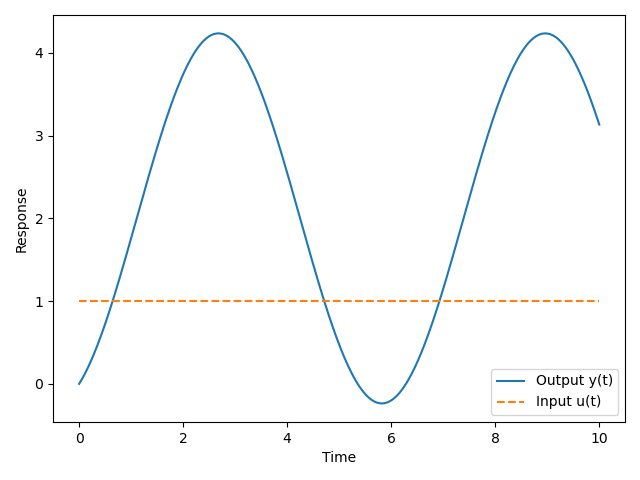
\includegraphics[scale=0.8]{../figures/first-degree-input-diffeq.png}
\end{center}

\subsection{Forma di Jordan}
Se gli autovalori sono multipli ma $A$ non è diagonalizzabile, abbiamo visto, occore sfruttare la \textbf{forma di Jordan} attraverso la trasformazione:
$$
J = Q A Q{-1}
$$
dove $Q$ è la matrice degli \textbf{autovettori generalizzati} con:
$$
J = \begin{pmatrix}
	J_1 & 0 & 0 \\
	0 & ... & 0 \\
	0 & 0 & J_N
\end{pmatrix}
$$
dove ogni $J_i$ è detto \textbf{miniblocco di Jordan}:
$$
J_i = \begin{pmatrix}
	\lambda_h & 1 & 0 & ... & 0 \\ 
	0 & \lambda_h & 1 & ... & 0 \\ 
	... & ... & ... & ... & ... \\ 
	0 & 0 & ... & \lambda_h & 1 \\
	0 & 0 & ... & 0 & \lambda_h
\end{pmatrix}
$$

Ogni blocco di Jordan ha sulla diagonale lo stesso autovalore, che compare tante volte quanto è la sua \textit{molteplicità algebrica}.
Inoltre, ci sono tanti blocchi $J_i$ associati allo stesso autovattore tante volte quanto è la sua \textit{molteplicità geometrica}.

\par\smallskip

Se riprendiamo la matrice esponenziale abbiamo:
$$
e^{At} = e^{QJQ^{-1}t} = Q \left( I + Jt + \frac{J^2 t^2}{2!} + ... + \frac{(Jt)^n}{n!} \right) Q^{-1} = Q e^{Jt} Q^{-1}
$$
dove $e^{Jt}$ è \textit{diagonale a blocchi}:
$$
e^{Jt} = \begin{pmatrix}
e^{J_1 t} & 0 & ... & 0 \\
0 & e^{J_2 t} & ... & 0 \\
... & ... & ... & ... \\ 
0 & ... & 0 ... & e^{J_n t}
\end{pmatrix}
$$
dove ogni blocco $e^{J_i t}$ ha la forma:
$$
e^{J_i t} = e^{ \begin{pmatrix}
		\lambda & 1 & 0 \\
		0 & ... & 1 \\ 
		0 & 0 & \lambda
\end{pmatrix} t}
= e^{(\lambda I + J_{0i})t} = e^{\lambda t} e^{J_{0i} t}
$$
dove con $J_{0i}$ ci riferiamo alla \textbf{parte nilpotente} di $J_i$.
Il problema sarà quindi capire la forma di $e^{J_{0i} t}$:
$$
e^{J_{0i} t} = I + J_{0i}t + \frac{J_{0i}^2}{2!} + ... + \frac{J_{0i}^{q - i} t^{q - 1}}{(q - 1)!}
$$
dove ogni coefficiente moltiplicativo di $t^i$ ha la proprietà di avere le entrate spostate in diagonale, verso l'alto a destra, per cui:
$$
e^{J_{0i} t} = \begin{pmatrix}
	1 & t & \frac{t^2}{2} & ... & \frac{t^{(q - 1)}}{(q - 1)!} \\
	0 & 1 & t & ... & ... \\
	0 & 0 & 1 & t & \frac{t^2}{2} \\ 
	0 & 0 & 0 & 1 & t \\
	0 & 0 & 0 & 0 & 1
\end{pmatrix}
$$
e quindi i modi del sistema sarano:
$$
t^k \frac{e^{\lambda t}}{k!}, \quad 0 \leq k \leq q - 1
$$
dove abbiamo finalmente capito il significato dell'intero $k$.

\par\smallskip
Notiamo che la proprietà di similarità che avevamo trovato:
$$
M = \begin{pmatrix}
	\sigma + j\omega & 0 \\
	0 & \sigma - j\omega
\end{pmatrix}
\sim
S = \begin{pmatrix}
	\sigma & \omega \\
	-\omega & \sigma
\end{pmatrix}
$$
ha un equivalente per le matrici in forma di Jordan:
$$
M=
\begin{pmatrix}
	\sigma + j \omega & 1 & 0 & 0 \\
	0 & \sigma + j \omega & 0 & 0 \\
	0 & 0 & \sigma - j \omega & 1 \\
	0 & 0 & 0 & \sigma - j \omega
\end{pmatrix}
\sim 
S=
\begin{pmatrix}
	\sigma & \omega & 1 & 0 \\
	-\omega & \sigma & 0 & 1 \\
	0 & 0 & \sigma & \omega \\
	0 & 0 & -\omega & \sigma \\
\end{pmatrix}
$$

e via dicendo.

\subsection{Stabilità nei sistemi lineari stazionari}
Riprendiamo la definizione di \textit{stabilità} (3.3 e 3.4).
Quello che interessa sono le \textbf{perturbazioni} dello stato.

Per un sistema lineare e stazionario l'origine è sempre punto di equilibrio per ingresso nullo.
Se l'origine è stabile, allora lo è qualsiasi altro punto di equilibrio.
Si può allore dire che un sistema è \textbf{stabile} solo guardando alla risposta \textit{libera} del sistema:
$$
x' = Ax + Bu, \quad u = 0, \quad x(0) = x_0
$$
$$
x(t) = e^{At}x_0
$$

In particolare, la stabilità del sistema dipende dai \textit{modi propri} del sistema.
In particolare, se gli autovalori hanno parte reale $\mathrm{Re}(\lambda_i) < 0$ il sistema è \textbf{asintoticamente stabile}, mentre se hanno parte reale $\mathrm{Re}(\lambda_i) \leq 0$ e gli $\mathrm{Re}(\lambda_i) = 0$ hanno molteplicità $\mu =1$ il sistema è solo \textbf{stabile}.
Quest'ultimo caso è propriamente quello delle matrici non diagonalizzabili (quindi messe in forma di Jordan).

Possiamo riassumere la relazione fra stabilità, modi e autovalori come segue:
\begin{table}[H]
	\center \rowcolors{2}{white}{black!10}
	\begin{tabular} { p{3.5cm} | p{5cm} | p{5cm} }
		\bfseries Stabilità & \bfseries Modi & \bfseries Autovalori \\
		\hline
		Stabilità asintotica & Tendono a zero & $\mathrm{Re}(\lambda_i) < 0$ \\
	Stabilità semplice o marginale & Non vanno a infinito, ma almeno uno non converge a zero & $\mathrm{Re}(\lambda_i) \leq 0$, $\exists \lambda_i^* : \mathrm{Re}(\lambda_i^*) = 0$, $\mu = 1$ \\
Instabilità & Almeno uno va a infinito & $\mathrm{Re}(\lambda_i) > 0$ o $\exists \lambda_i^* : \mathrm{Re}(\lambda_i^*)$, $\mu_a(\lambda_i^*) \neq \mu_g(\lambda_i^*)$ \\
	\end{tabular}
\end{table}

\subsubsection{Stabilità dei sistemi linearizzati}
Avevamo visto che nei sistemi non lineari conviene \textit{linearizzare} trascurando i termini oltre il primo ordine nell'intorno di uno stato di equilibrio noto.
Se il sistema linearizzato è \textit{asintoticamente stabile}, si avrà che lo stato di equilibrio del sistema non lineare è \textbf{stabile}.
Di contro, se il sistema linearizzato è \textit{semplicemente stabile} non possiamo concludere nulla sul sistema non lineare (potrebbero esserci instabilità ai termini superiori).

\end{document}
